\chapter{Implementierung} \label{cha:implementierung}

\section{Entwickeln der Hunt-Editor Web-App}

\subsection{Organisation}

\begin{figure}[H]
  \centering
  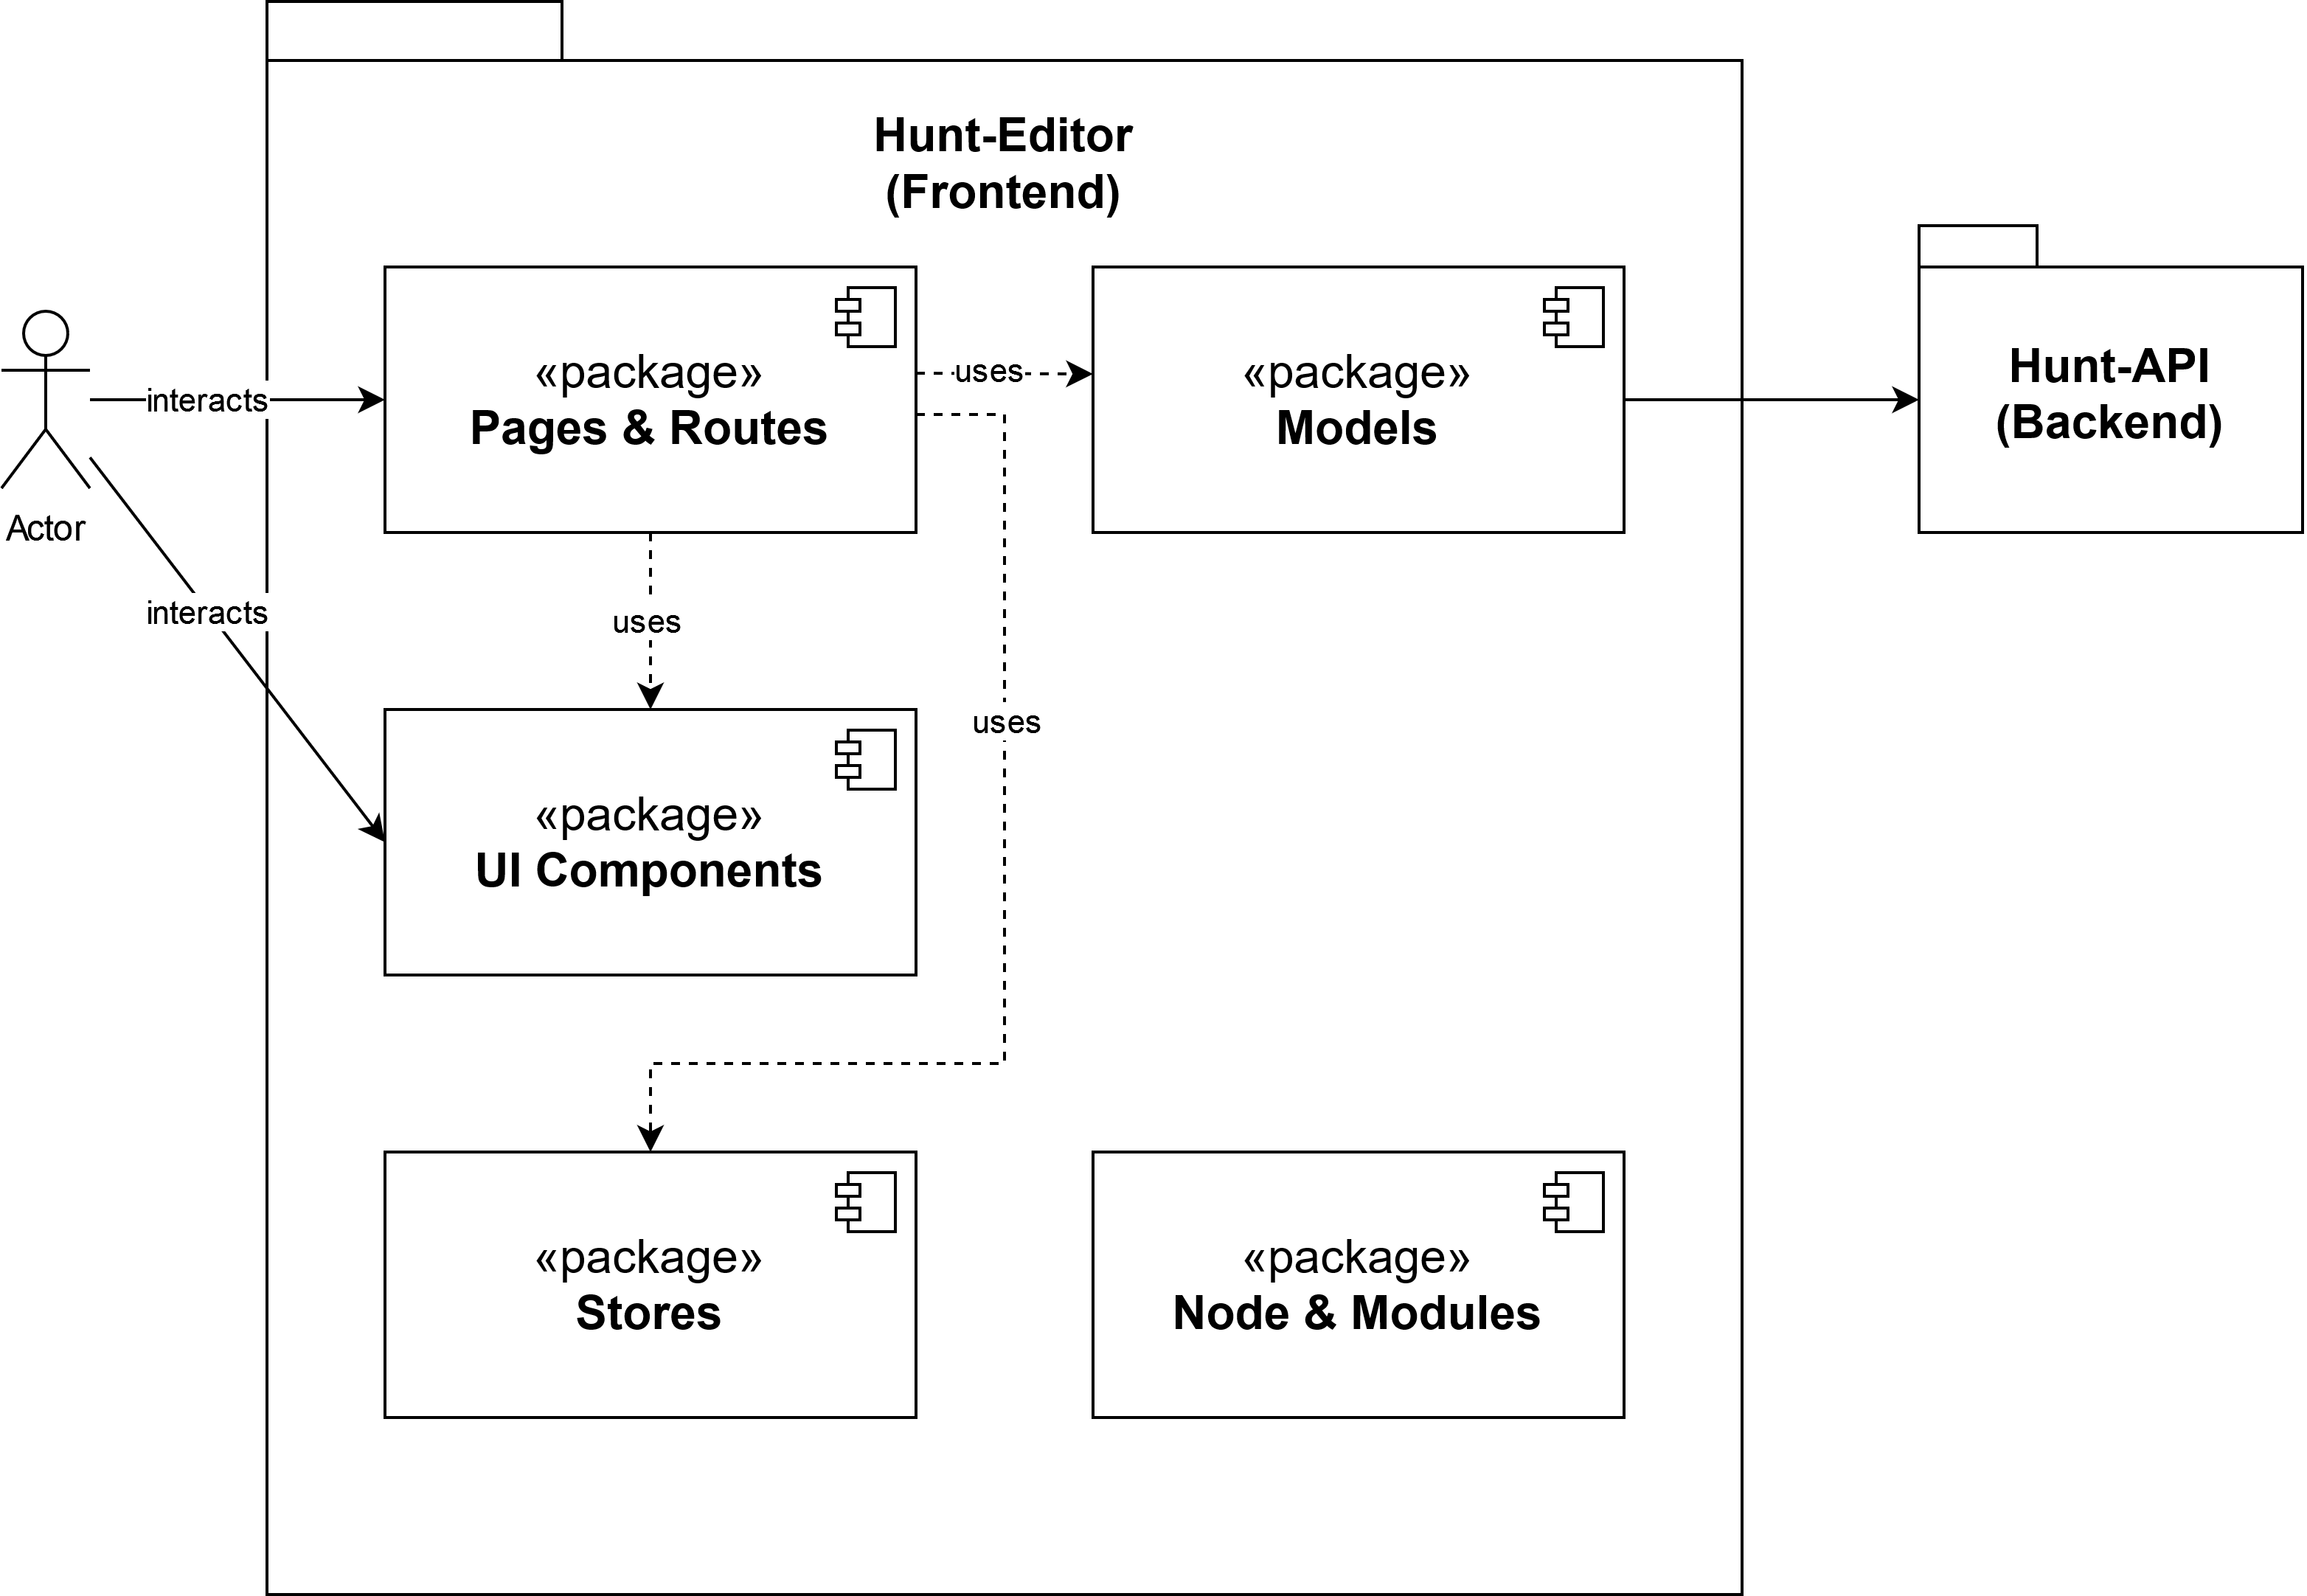
\includegraphics[width=1\textwidth]{images/PrAR-Loesung-Hunt-Editor-Components.png}
  \caption{UML-Diagramm Whitebox Frontend Hunt-Editor}
  \label{fig:whitebox-frontend}
\end{figure}

Abbildung \ref{fig:whitebox-frontend} skizziert die grundlegenden Elemente, aus welchen die Anwendung besteht. Für das Zwischenspeichern der Schnitzeljagd-Attribute (Titel, Beschreibung, Aufgaben) werden Svelte Stores verwendet (vgl. Kapitel \ref{cha:grundlagen:swtech:svelte}).

Im Folgenden ist die Struktur des Routings als Baumdiagramm dargestellt. Wie eine Svelte-Anwendung aufgebaut ist, wird in Kapitel \ref{cha:grundlagen:swtech:svelte} näher beschrieben.

\begin{figure}[H]
  \centering
  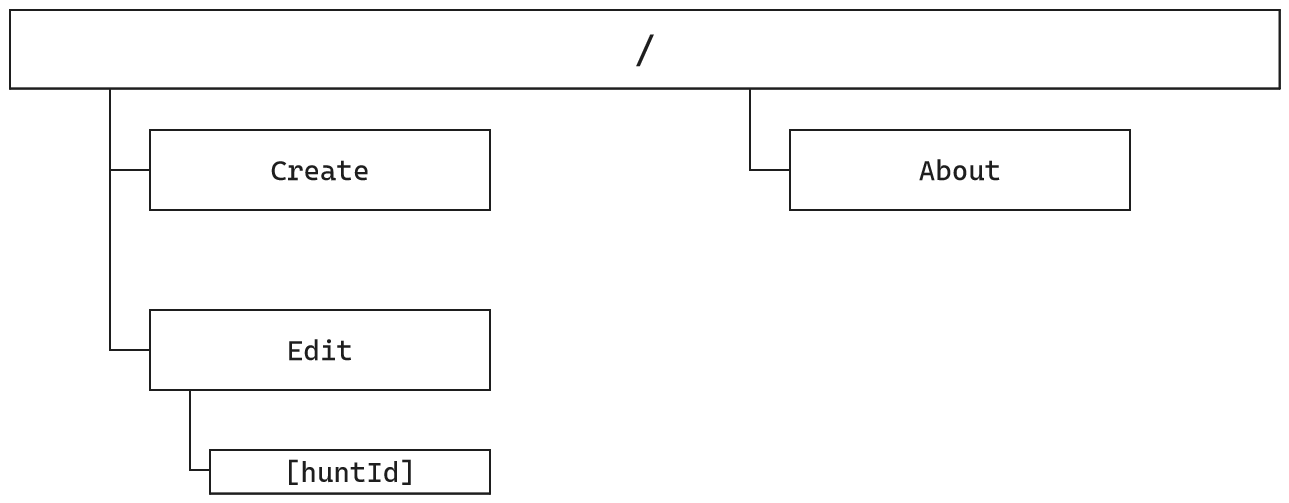
\includegraphics[width=1\textwidth]{images/PrAR-Loesung-Hunt-Editor-Routes.png}
  \caption{Skizze Frontend Hunt-Editor Routes}
  \label{fig:frontend-routes}
\end{figure}

Für das Anzeigen und Entfernen von Schnitzeljagden ist die Home Route \textit{/} vorgesehen. Auf der Route \textit{/about} werden Informationen zur Anwendung und zum Projekt bereitgestellt.

Der Workflow zum Erstellen einer Schnitzeljagd ist in der Route \textit{/create} implementiert.

Zum Editieren einer Schnitzeljagd werden die Komponenten aus der \textit{/create}-Route wiederverwendet, hier wird jedoch über die \textit{/edit/[huntId]}-Route gearbeitet, wobei \textit{[huntId]} ein Platzhalter für die \textit{Id} der jeweiligen Schnitzeljagd ist. Dadurch können dynamisch über die URL Informationen zur Schnitzeljagd abgerufen werden. Diese Informationen (wie bspw. Titel und Beschreibung) werden dann in die Eingabefelder eingetragen.

\subsection{UI-Design}

Um den Editor zu erstellen, wurde zunächst versucht, mit DaisyUI zu arbeiten. Da dies nicht das gewünschte Ergebnis geliefert hat, wurde zu Flowbite gewechselt. Kapitel \ref{appendix:adr:daisy} begründet diese Entscheidung.

\section{Entwickeln einer AR-Anwendung mit Unity und AR-Foundation} \label{cha:implementierung:unityardev}

Im Folgenden ist der Entwicklungsprozess für das Implementieren eines AR-Image-Trackers mithilfe des AR-Foundation Frameworks von Unity beschrieben. Im Anschluss wird erläutert, weshalb dieser Ansatz für das Projekt obsolet wurde.

Für die Entwicklung mit Unity wird die Installation des Unity-Hubs und einer unterstützten Version des Unity-Editor vorausgesetzt. Die im Projekt entwickelte Anwendung wurde mit der Editor-Version \textit{2022.3.20f1} erstellt.

\subsection{Anlegen einer Reference-Image-Library}

Nachdem ein AR-Unity-Projekt nach \autocite{Unity2024:ProjectSetup} angelegt wurde und das nötige Framework eingebunden wurde, stehen verschiedene Funktionen des AR-Foundation-Frameworks im Editor zur Verfügung.

Zunächst soll eine \textit{Reference-Image-Library} erstellt werden. Abbildung \ref{fig:implementierung:unity:AR-Create-Img-Lib} markiert die grundlegenden Schritte hierfür.

\begin{figure}[H]
    \centering
    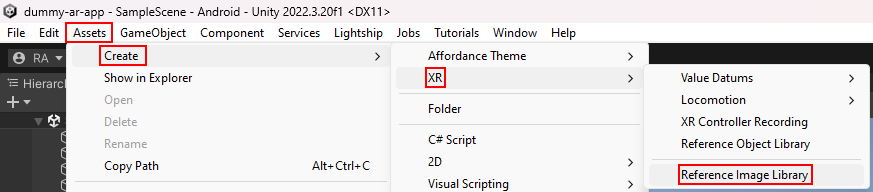
\includegraphics[width=\textwidth]{images/PrAr_UnityAR-Create-Img-Lib.png}
    \caption{Bildschirmabschnitt für das Erstellen einer Reference-Image-Library}
    \label{fig:implementierung:unity:AR-Create-Img-Lib}
\end{figure}

In der geöffneten Szene in Abbildung \ref{fig:implementierung:unity:AR-See-Img-Lib} sollte nun ein leeres Reference-Image-Library Objekt existieren.

\begin{figure}[H]
    \centering
    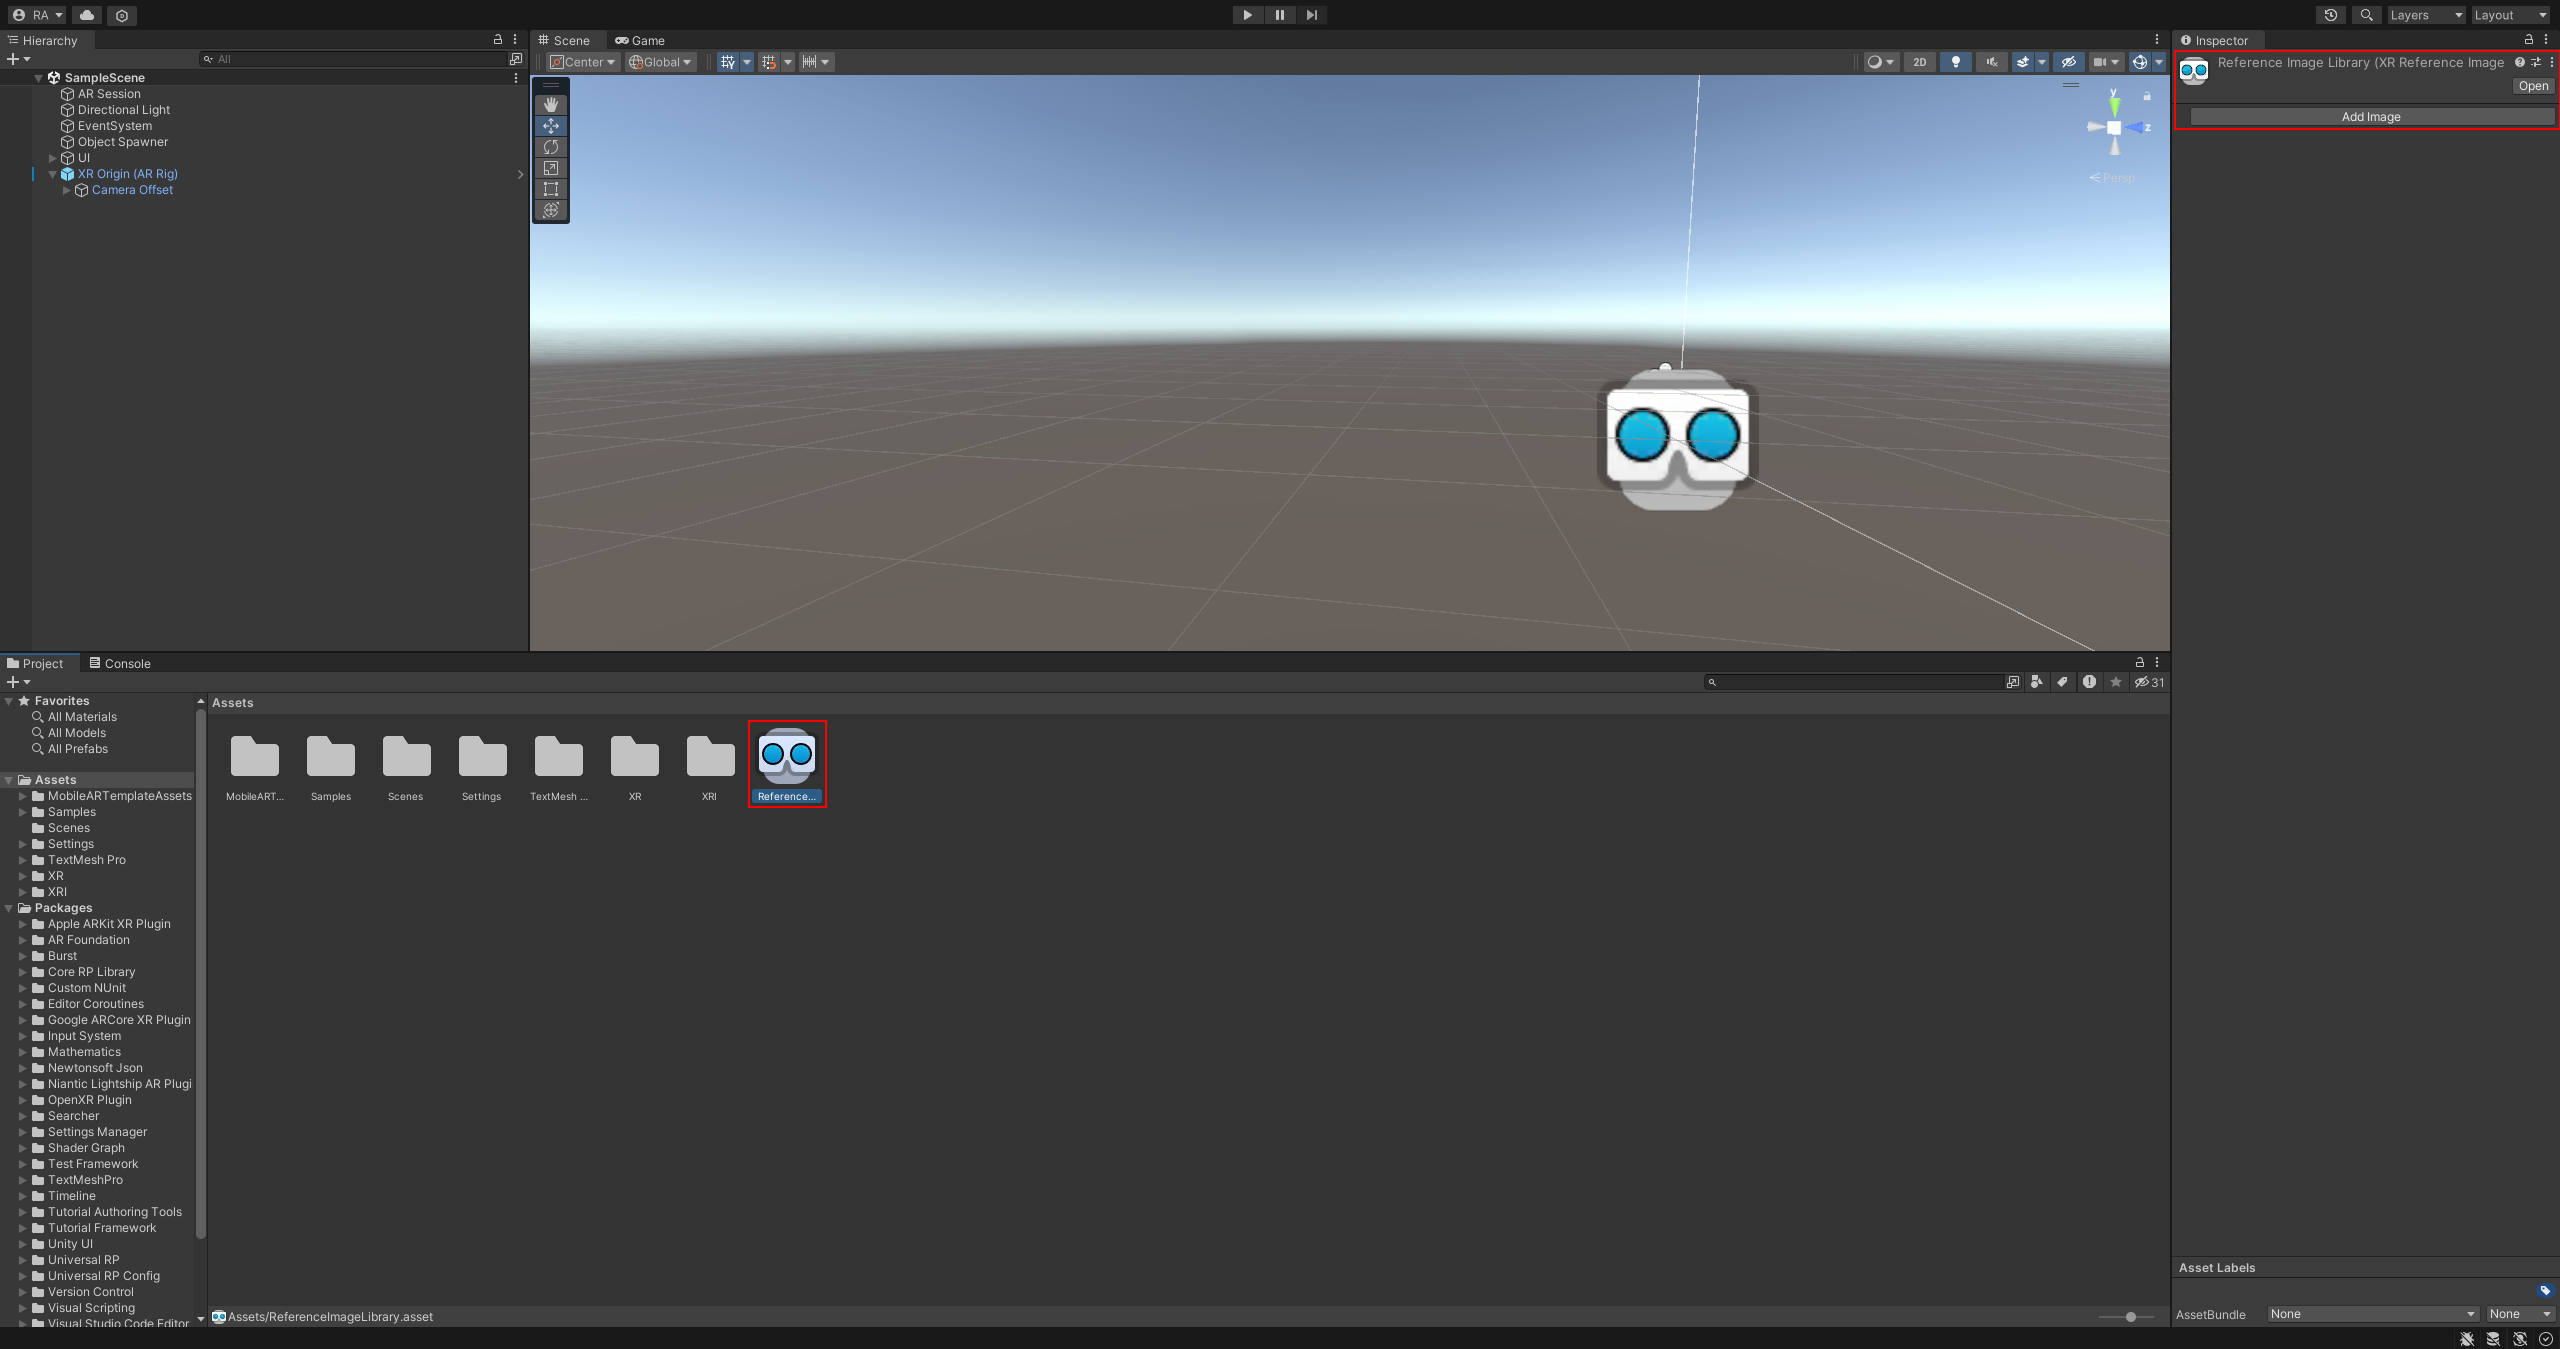
\includegraphics[width=\textwidth]{images/PrAr_UnityAR-See-Img-lib.png}
    \caption{Bildschirmabschnitt Reference-Image-Library Objekt im Editor}
    \label{fig:implementierung:unity:AR-See-Img-Lib}
\end{figure}

Die Reference-Image-Library wird benötigt, um vor der Laufzeit bereits Referenzbilder (\textit{Reference-Images}) oder Objekte zu sammeln, die von einem AR-Tracker wie etwa die Komponente \textit{XRImageTrackingSubsystem} erkannt werden können.

\subsection{Anlegen eines AR-Tracked-Image-Managers}

Die \textit{AR Tracked Image Manager} Komponente erstellt \textit{Game-Objects} für jedes gefundene Bild innerhalb des Viewports des Benutzers. Bevor ein Bild gefunden werden kann, muss die Komponente Referenz-Bilder kennen, die in der \textit{Reference-Image-Library} gespeichert sind.

Das Einbinden erfolgt, indem ein Skript an die XR-Origin Komponente angebunden wird und die dementsprechende Reference-Image-Library per Drag-and-Drop eingebunden wird. Dies aktiviert das Tracken von Bildern im AR-Raum.

\begin{figure}[H]
    \centering
    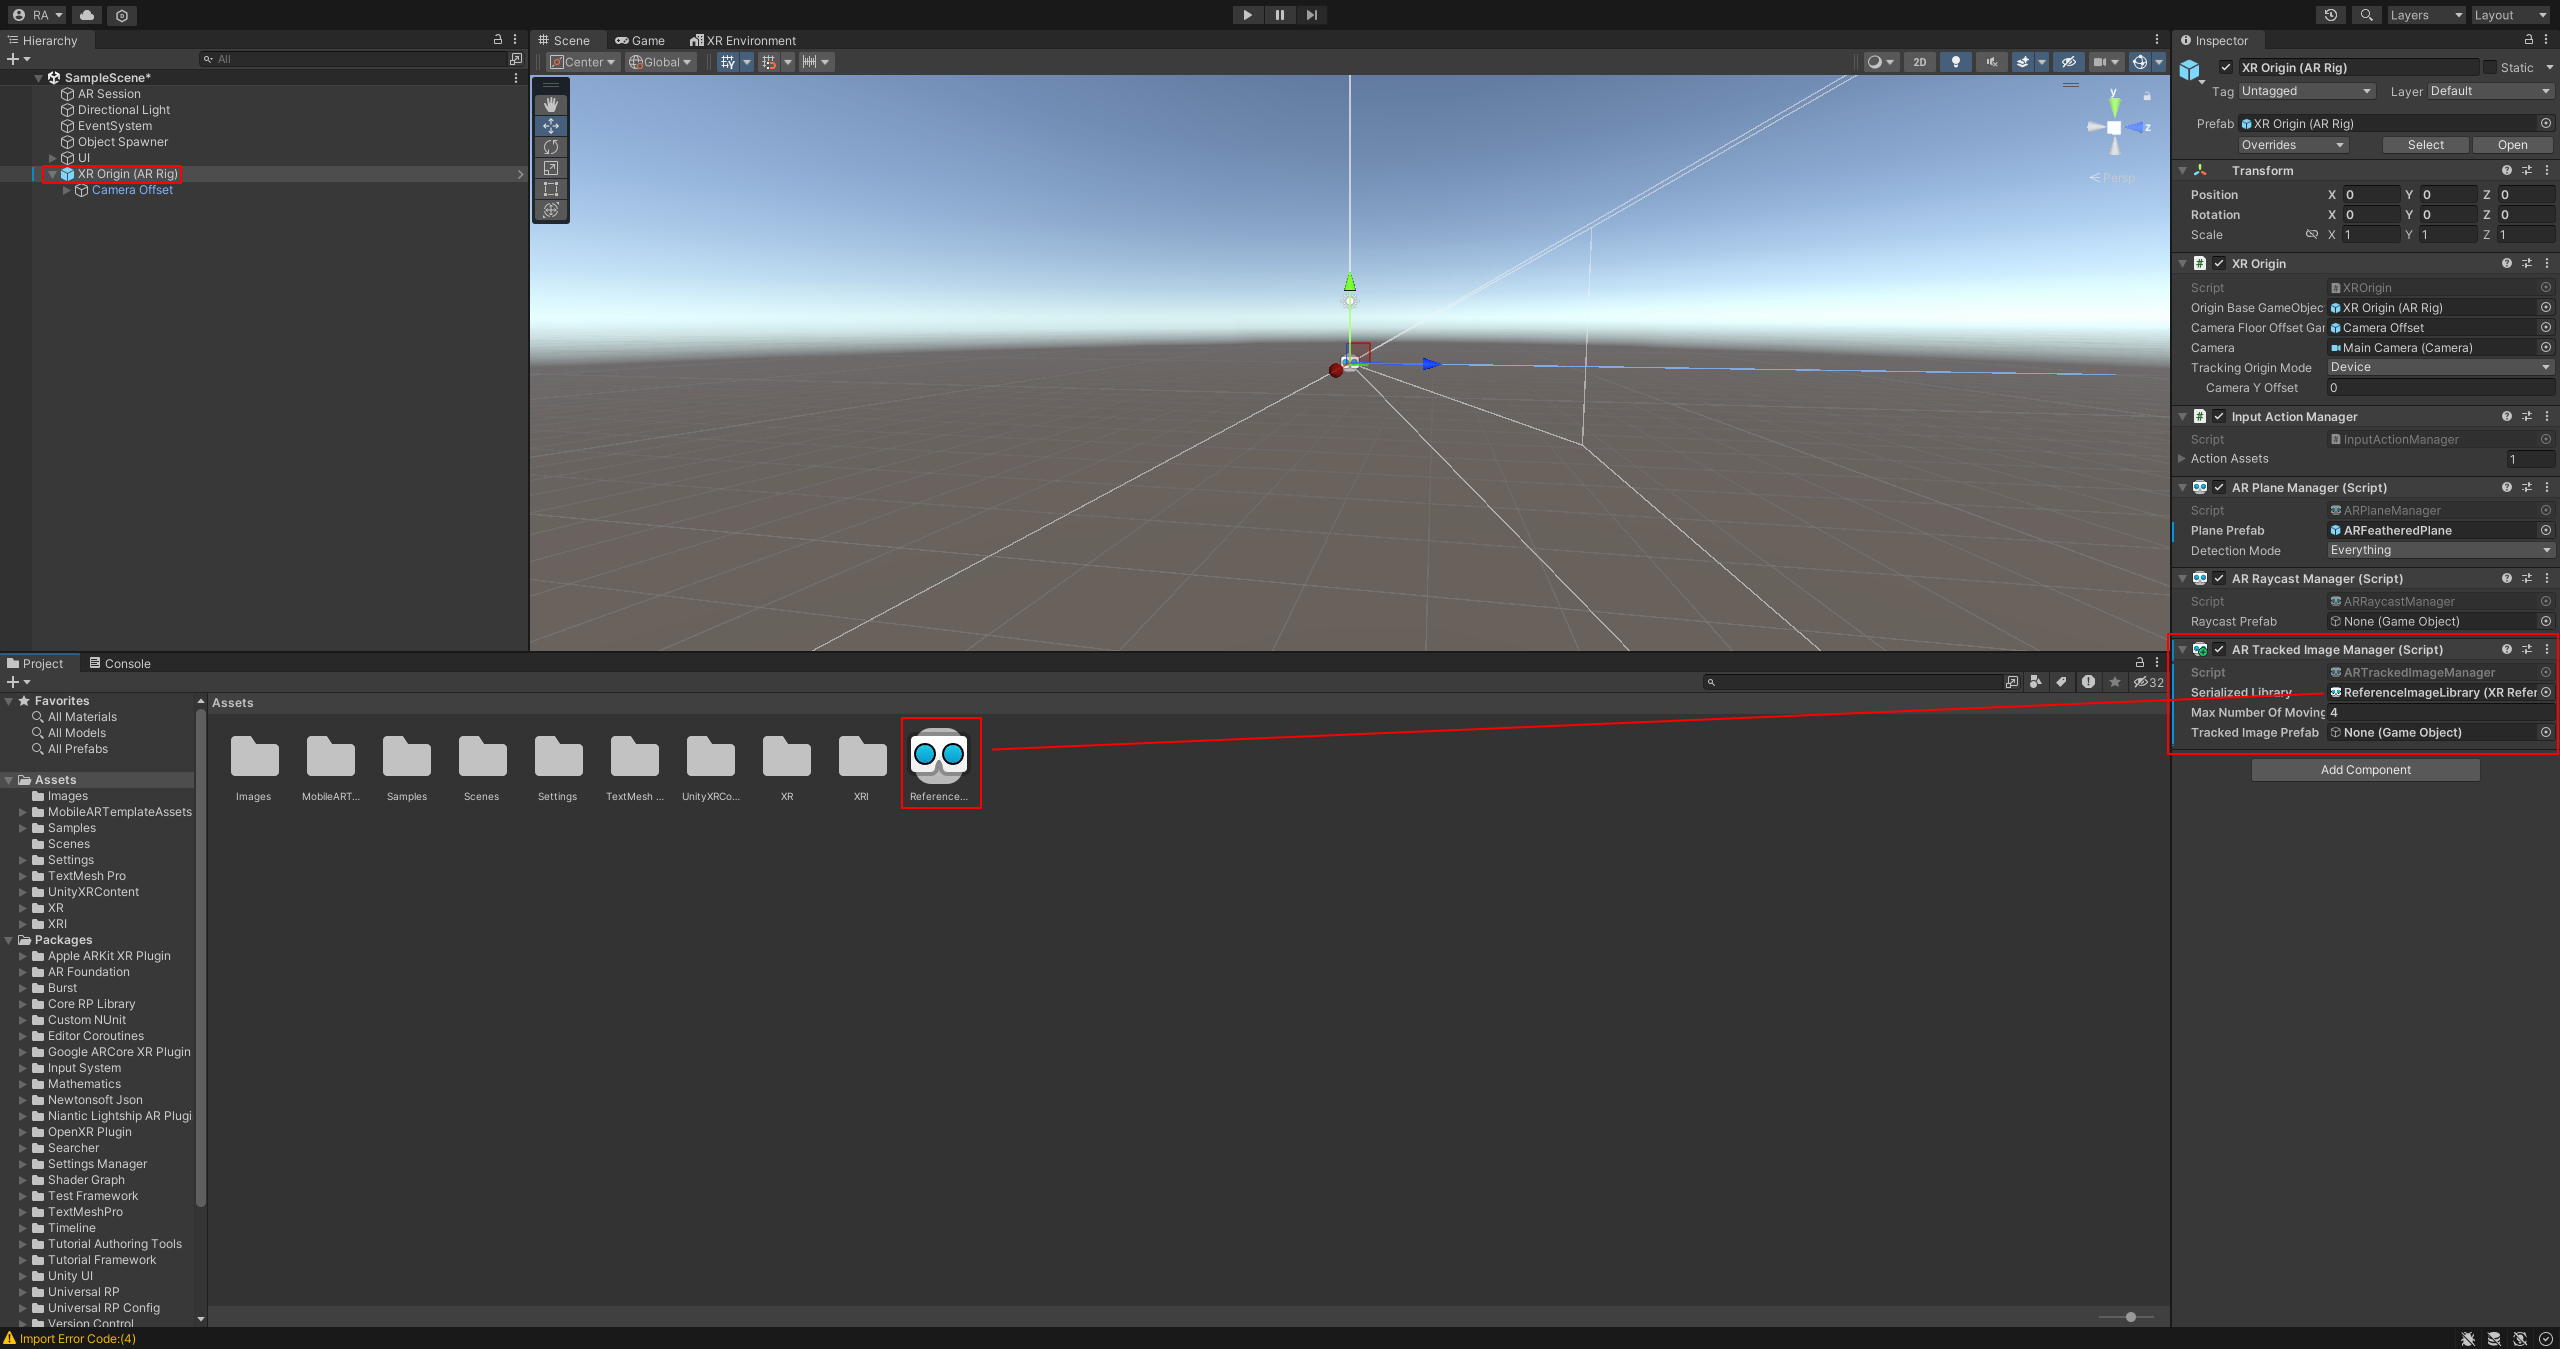
\includegraphics[width=\textwidth]{images/PrAr_UnityAR-Create-Img-Mngr.png}
    \caption{Bildschirmabschnitt für das Erstellen eines AR-Tracked-Image-Managers}
    \label{fig:implementierung:unity:AR-Create-Img-Mngr}
\end{figure}

\subsection{QR-Code-Daten aus einem Referenz-Bild lesen}

Das erkennen eines QR-Codes erfordert, dass dieser in der Reference-Image-Library bereits angelegt wurde. Nachdem dies erfolgt ist, kann der QR-Code als Textur gelesen und über einen QR-Code-Konverter wie \textit{ZXing} als Text konvertiert werden. Abbildung \ref{fig:implementierung:unity:AR-Read-Qr-Img} zeigt das erfolgreiche Umkonvertieren eines QR-Codes im AR-Raum.

\begin{figure}[H]
    \centering
    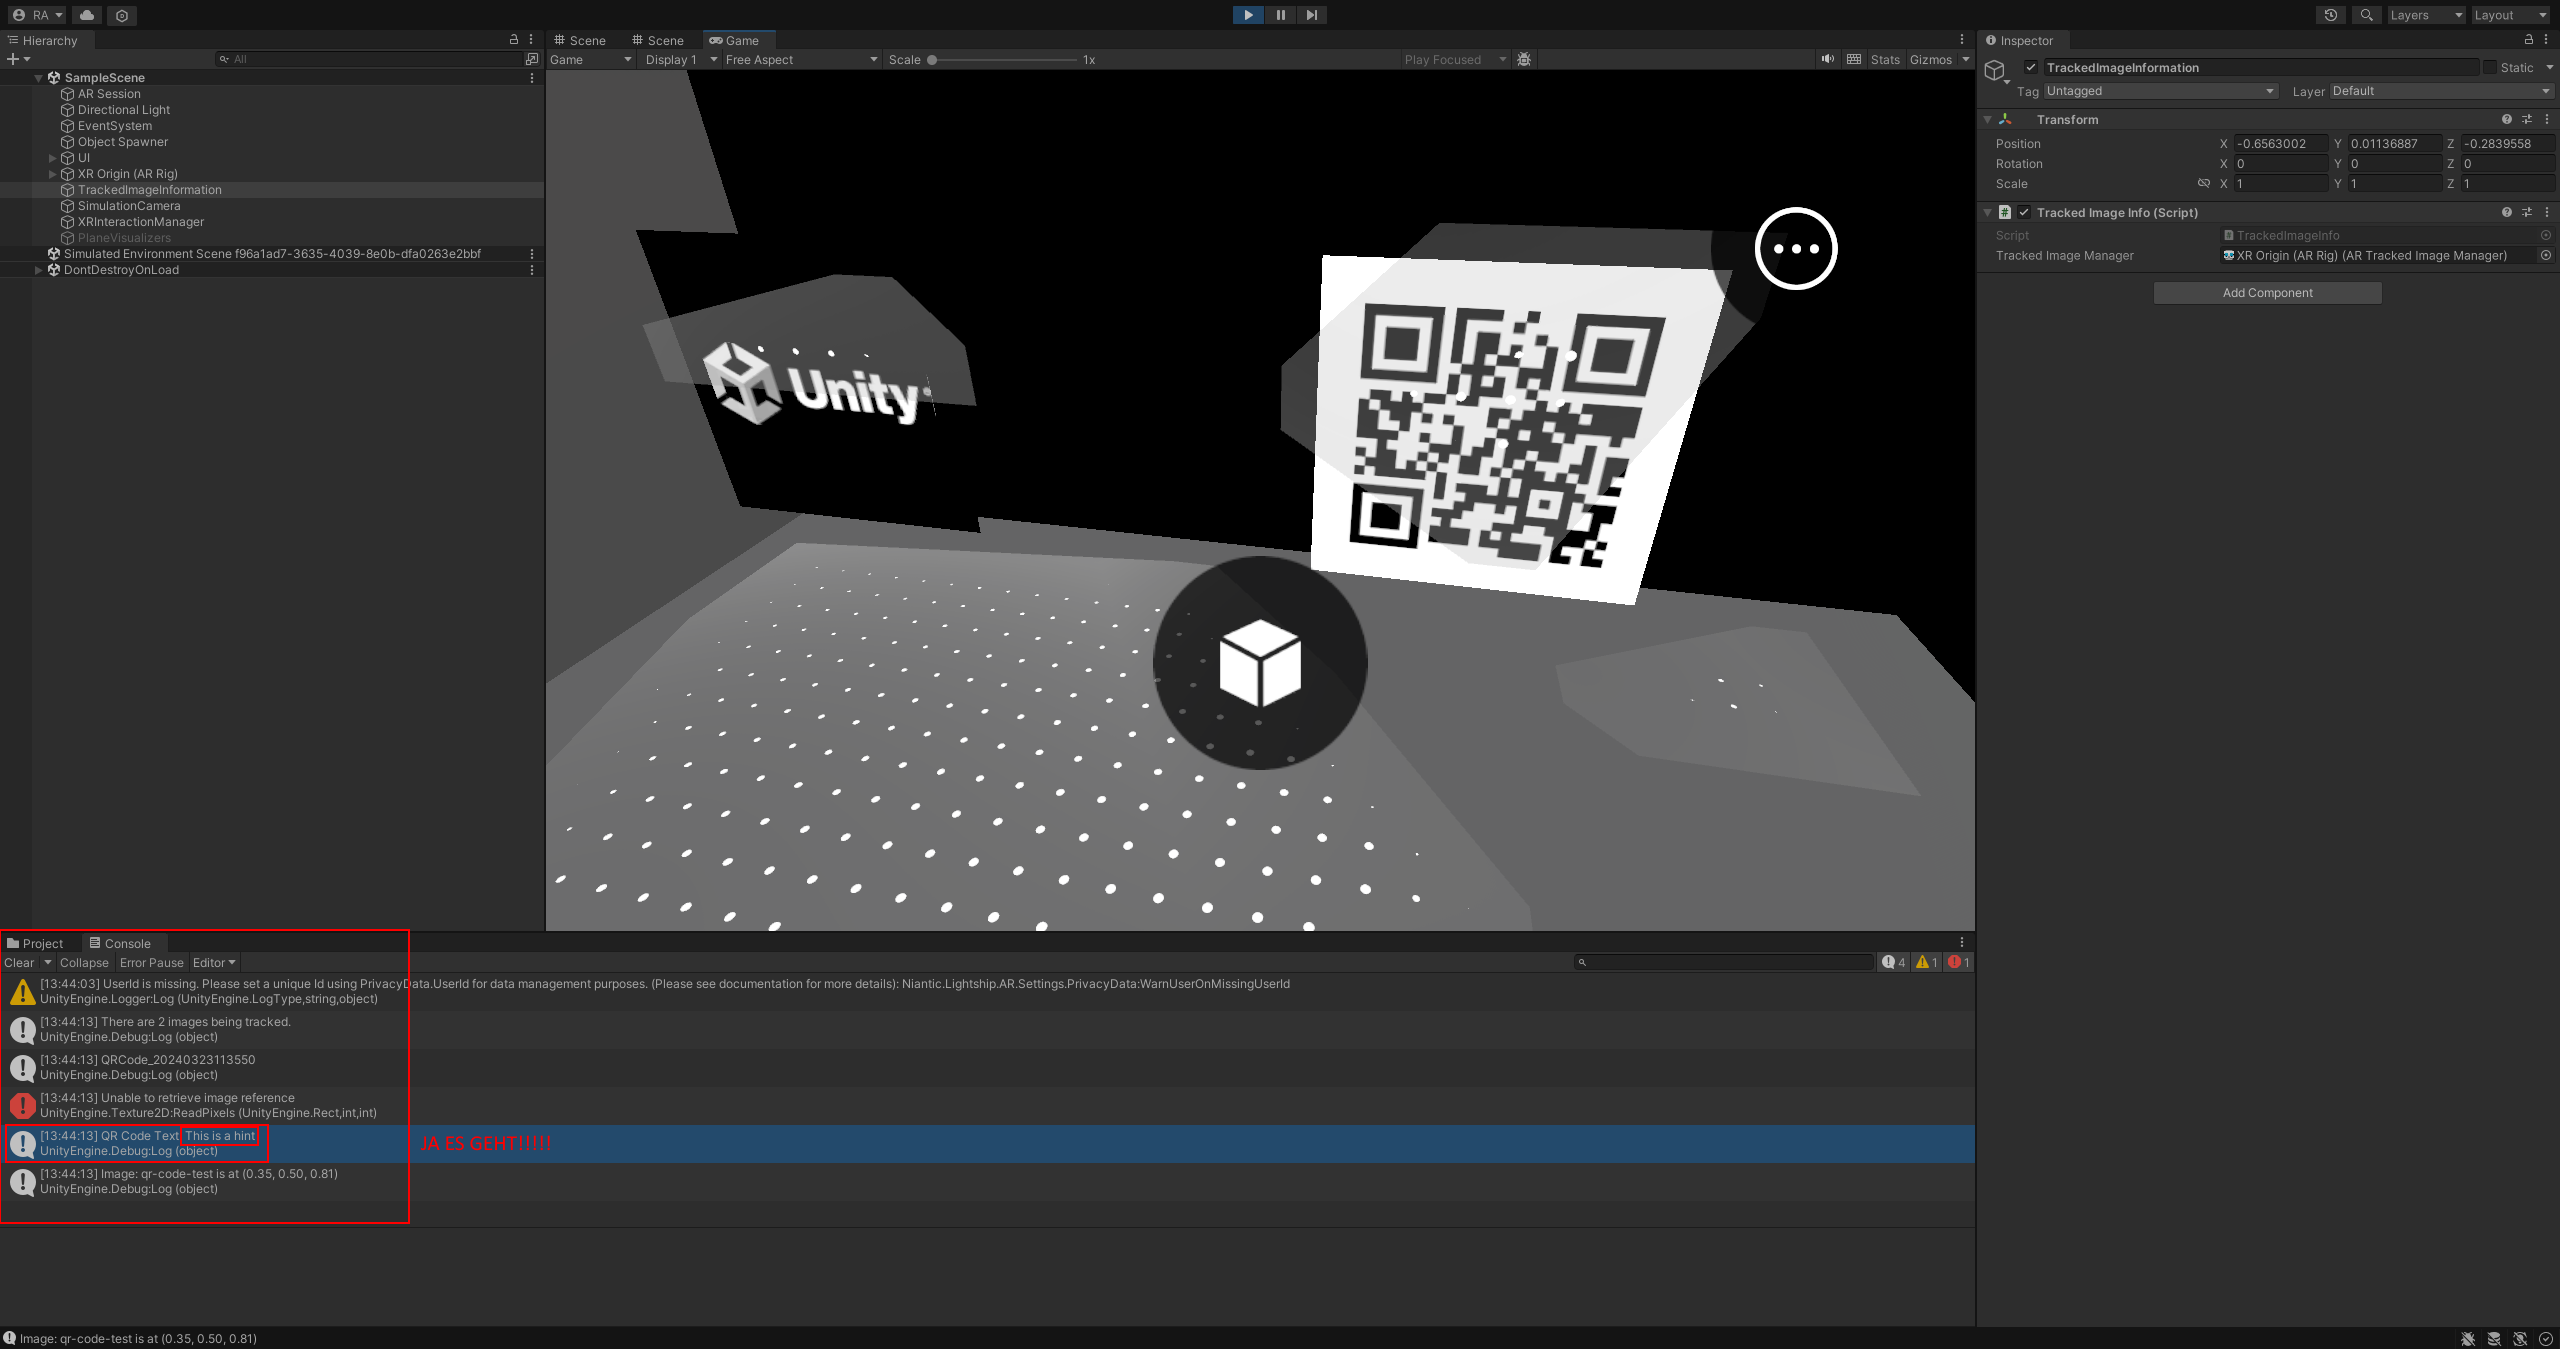
\includegraphics[width=\textwidth]{images/PrAr_UnityAR-Read-Qr-Img.png}
    \caption{Bildschirmabschnitt für das Lesen eines QR-Codes}
    \label{fig:implementierung:unity:AR-Read-Qr-Img}
\end{figure}

\subsection{Erfahrung mit Unity und AR-Foundation}

Leider kann über den in Kapitel \ref{cha:implementierung:unityardev} beschriebenen Ansatz kein gewünschtes Ergebnis erzielt werden.

Ein Hinweistext oder -bild an der Position des QR-Codes zu platzieren, könnte theoretisch funktionieren, wie in Abbildung \ref{fig:implementierung:unity:AR-Read-Qr-Img} bereits dargestellt wird. Allerdings stellt die mangelnde Flexibilität der Reference-Image-Library ein erhebliches Hindernis für eine funktionierende Implementierung dar.

Um dieses Problem zu umgehen, müsste die Anwendung beim Start alle im System vorhandenen QR-Codes und ihre entsprechenden Lösungen über das Backend abrufen. Dies würde jedoch bei einer großen Anzahl von QR-Codes zu einer suboptimalen Benutzererfahrung führen, da die Anwendung erheblich verzögert wäre. Zusätzlich verursacht das Laden mehrerer QR-Codes einen hohen Speicheraufwand. 

Außerdem werden die Lösungen vor dem Erhalt eines ersten Hinweises auf dem Gerät des Teilnehmers geladen. Dies könnte zur Folge haben, dass manche Lösungen aus den geladenen Bildern extrahiert werden können, wodurch das Konzept der Schnitzeljagd umgangen wird.

Diese Herausforderungen zeigen deutlich, dass Unity und AR Foundation in diesem Kontext nicht die optimale Lösung darstellen. Die genannten Einschränkungen machen es schwierig, eine flexible, effiziente und sichere Anwendung zu entwickeln, die den Anforderungen einer Schnitzeljagd entspricht. Daher ist es ratsam, alternative Technologien oder Ansätze zu berücksichtigen, die eine bessere Anpassungsfähigkeit und Sicherheit bieten.

Die Entscheidung, Unity nicht für das Schnitzeljagd-Spiel zu verwenden, wird zudem in folgenden Aspekten begründet.

\subsubsection{Entwicklungsumgebung und Tooling}

Die Entwicklungsumgebung und der Entwicklungsprozess, die für die Erstellung einer Anwendung in Unity erforderlich sind, weisen erhebliche Nachteile auf. Das Tooling von Unity ist oft unhandlich und ineffizient. Häufig auftretende Probleme müssen durch Neustarts des Unity-Hubs oder des Unity-Editors gelöst werden. Diese häufigen Unterbrechungen führen zu einem erheblichen Zeitverlust, der den Entwicklungsprozess stark behindert.

Ein weiteres Problem ist die resultierende Größe der Anwendung nach dem Build. Die Unity-Engine erzeugt sehr große Dateien, selbst wenn nur grundlegende Funktionen verwendet werden. Eine Optimierung auf das Nötigste ist kaum möglich, was die Anwendung unnötig aufbläht und somit unpraktisch für mobile Geräte macht.

\subsubsection{Anpassung auf Projektanforderungen}

AR Foundation, die AR-Entwicklungsplattform von Unity, bietet für unsere Schnitzeljagd-Anwendung keine entscheidenden Vorteile. Unsere Anwendung konzentriert sich hauptsächlich auf die Darstellung von Texten und Bildern sowie das Scannen von QR-Codes, was keine umfassende AR-Funktionalität erfordert. Eine einfache und ressourcenschonende Lösung wäre hier weitaus effizienter.

\subsubsection{Lizensierung und Business}

Das Unternehmen hinter Unity, Unity Technologies, hat in den letzten Monaten erheblich an Reputation verloren. Grund dafür sind umstrittene Änderungen in den Lizenzbedingungen und Preismodellen. Diese Änderungen haben bei Entwicklern für Unmut gesorgt und das Vertrauen in das Unternehmen erschüttert. \autocite{Unity2024:PriceChange}

Die negativen Schlagzeilen und die Unsicherheit über zukünftige Geschäftsstrategien machen Unity zu einer risikobehafteten Wahl für langfristige Projekte.

\subsection{Alternativen}

\subsubsection{Vuforia}
% TODO: eigentlich auch bescheuert da Unity Editor trz verwendet wird als editor; oder man müsste Android studio lernen; außerdem hat das auch pricing mit drinne siehe https://www.ptc.com/en/products/vuforia/vuforia-engine/pricing; 
%-------------------------------------%
\subsubsection{WebAr}
Eine vielversprechende Alternative zur nativen AR-Entwicklung mit Unity ist WebAR. WebAR ermöglicht AR-Erlebnisse direkt im Webbrowser ohne die Notwendigkeit einer separaten App-Installation. Dies bietet mehrere Vorteile:
\begin{itemize}
    \item \textbf{Zugänglichkeit}: WebAR ist auf jedem modernen Webbrowser verfügbar, was die Zugänglichkeit für Benutzer erleichtert und die Notwendigkeit, eine spezielle App herunterzuladen, beseitigt. Dies kann die Benutzerfreundlichkeit und die Reichweite der Anwendung erhöhen.

    \item \textbf{Einfachere Entwicklung}: WebAR nutzt Web-Technologien wie JavaScript und WebGL, die für viele Entwickler vertrauter und zugänglicher sind als die speziellen Tools und Skripte von Unity. Die Entwicklung kann daher schneller und einfacher sein, besonders wenn bereits Erfahrung mit Web-Technologien besteht.

    \item \textbf{Kosteneffizienz}: Da WebAR keine zusätzlichen Lizenzgebühren oder Laufzeitgebühren erfordert, ist es eine kostengünstigere Lösung.

\end{itemize}

\subsubsection{Schlussfolgerung}
Falls die Schnitzeljagd Anwendung in Zukunft AR-Funktionen beinhalten soll, stellt WebAR die effizienteste und kostengünstigste Lösung dar. Es bietet eine einfache und zugängliche Möglichkeit, grundlegende AR-Funktionen bereitzustellen, ohne die Notwendigkeit für eine komplexe App-Installation oder hohe Entwicklungs- und Betriebskosten. Vuforia und Unity bieten erweiterte Funktionen, die für diese Anwendung nicht erforderlich sind und könnten daher überdimensioniert sein.

%------------------------------------%


\section{Algorithmen zur Hinweisbestimmung für Nutzerlösungen}

Um dem Nutzer Hinweise zu geben, dass eine von ihm eingesandte Lösung nahezu korrekt ist, wurden zwei Algorithmen implementiert. Diese Algorithmen helfen dabei, den Grad der Übereinstimmung zwischen der vom Nutzer angegebenen Lösung und der tatsächlich gesuchten Antwort zu bestimmen.

\subsection{Haversine-Algorithmus zur Bestimmung geografischer Distanzen}

Einer der Algorithmen kommt zum Einsatz, wenn die Lösung einen geografischen Ort umfasst, der durch Breiten- und Längengrade (Latitude und Longitude) definiert ist. Hier wird die Haversine-Formel verwendet, um die Entfernung zwischen den beiden Punkten zu berechnen.

Die Haversine-Formel ist besonders nützlich, um die kürzeste Entfernung über die Erdoberfläche zu bestimmen, da sie die Krümmung der Erde berücksichtigt. Diese Berechnung ist essenziell, um zu bestimmen, wie nahe ein Nutzer mit seiner Antwort an der korrekten Position liegt.

Der folgende C\#-Code zeigt die Implementierung des Haversine-Algorithmus:

\begin{lstlisting}[language=c, caption={Code Ausschnitt zum Haversine Algorithmus in C\#}]
public static double Haversine(double lat1, double lon1, double lat2, double lon2)
{
    // Convert degrees to radians
    double dLat = ToRadians(lat2 - lat1);
    double dLon = ToRadians(lon2 - lon1);

    lat1 = ToRadians(lat1);
    lat2 = ToRadians(lat2);

    // Haversine formula
    double a = Math.Sin(dLat / 2) * Math.Sin(dLat / 2) +
               Math.Sin(dLon / 2) * Math.Sin(dLon / 2) * Math.Cos(lat1) * Math.Cos(lat2);
    double c = 2 * Math.Atan2(Math.Sqrt(a), Math.Sqrt(1 - a));

    // Distance in meters
    return RADIUS_OF_EARTH_METERS * c;
}

private static double ToRadians(double angleInDegrees)
{
    return angleInDegrees * Math.PI / 180.0;
}
\end{lstlisting}

In diesem Algorithmus wird zunächst die Differenz zwischen den Längen- und Breitengraden der beiden Punkte berechnet und in Radianten umgewandelt. Anschließend wird die Haversine-Formel angewendet, um den Anteil des großen Kreises (die kürzeste Strecke zwischen zwei Punkten auf der Oberfläche einer Kugel) zu berechnen, den der Abstand zwischen den Punkten darstellt. Dieser Anteil wird dann mit dem Radius der Erde multipliziert, um die tatsächliche Entfernung in Metern zu erhalten.

Durch diese Berechnung kann das System bestimmen, wie weit der vom Nutzer angegebene Ort von der korrekten Position entfernt ist, und so ein Feedback geben, das darauf hinweist, dass die Lösung nahe dran ist, wenn der Abstand gering ist.

\subsubsection{Anwendungsbeispiel des Haversine-Algorithmus}

Im folgenden wird der Harvesine-Algorithmus zum Bestimmen der Distanz des Benutzers zur Lösung verwendet.

\begin{figure}[H]
    \centering
    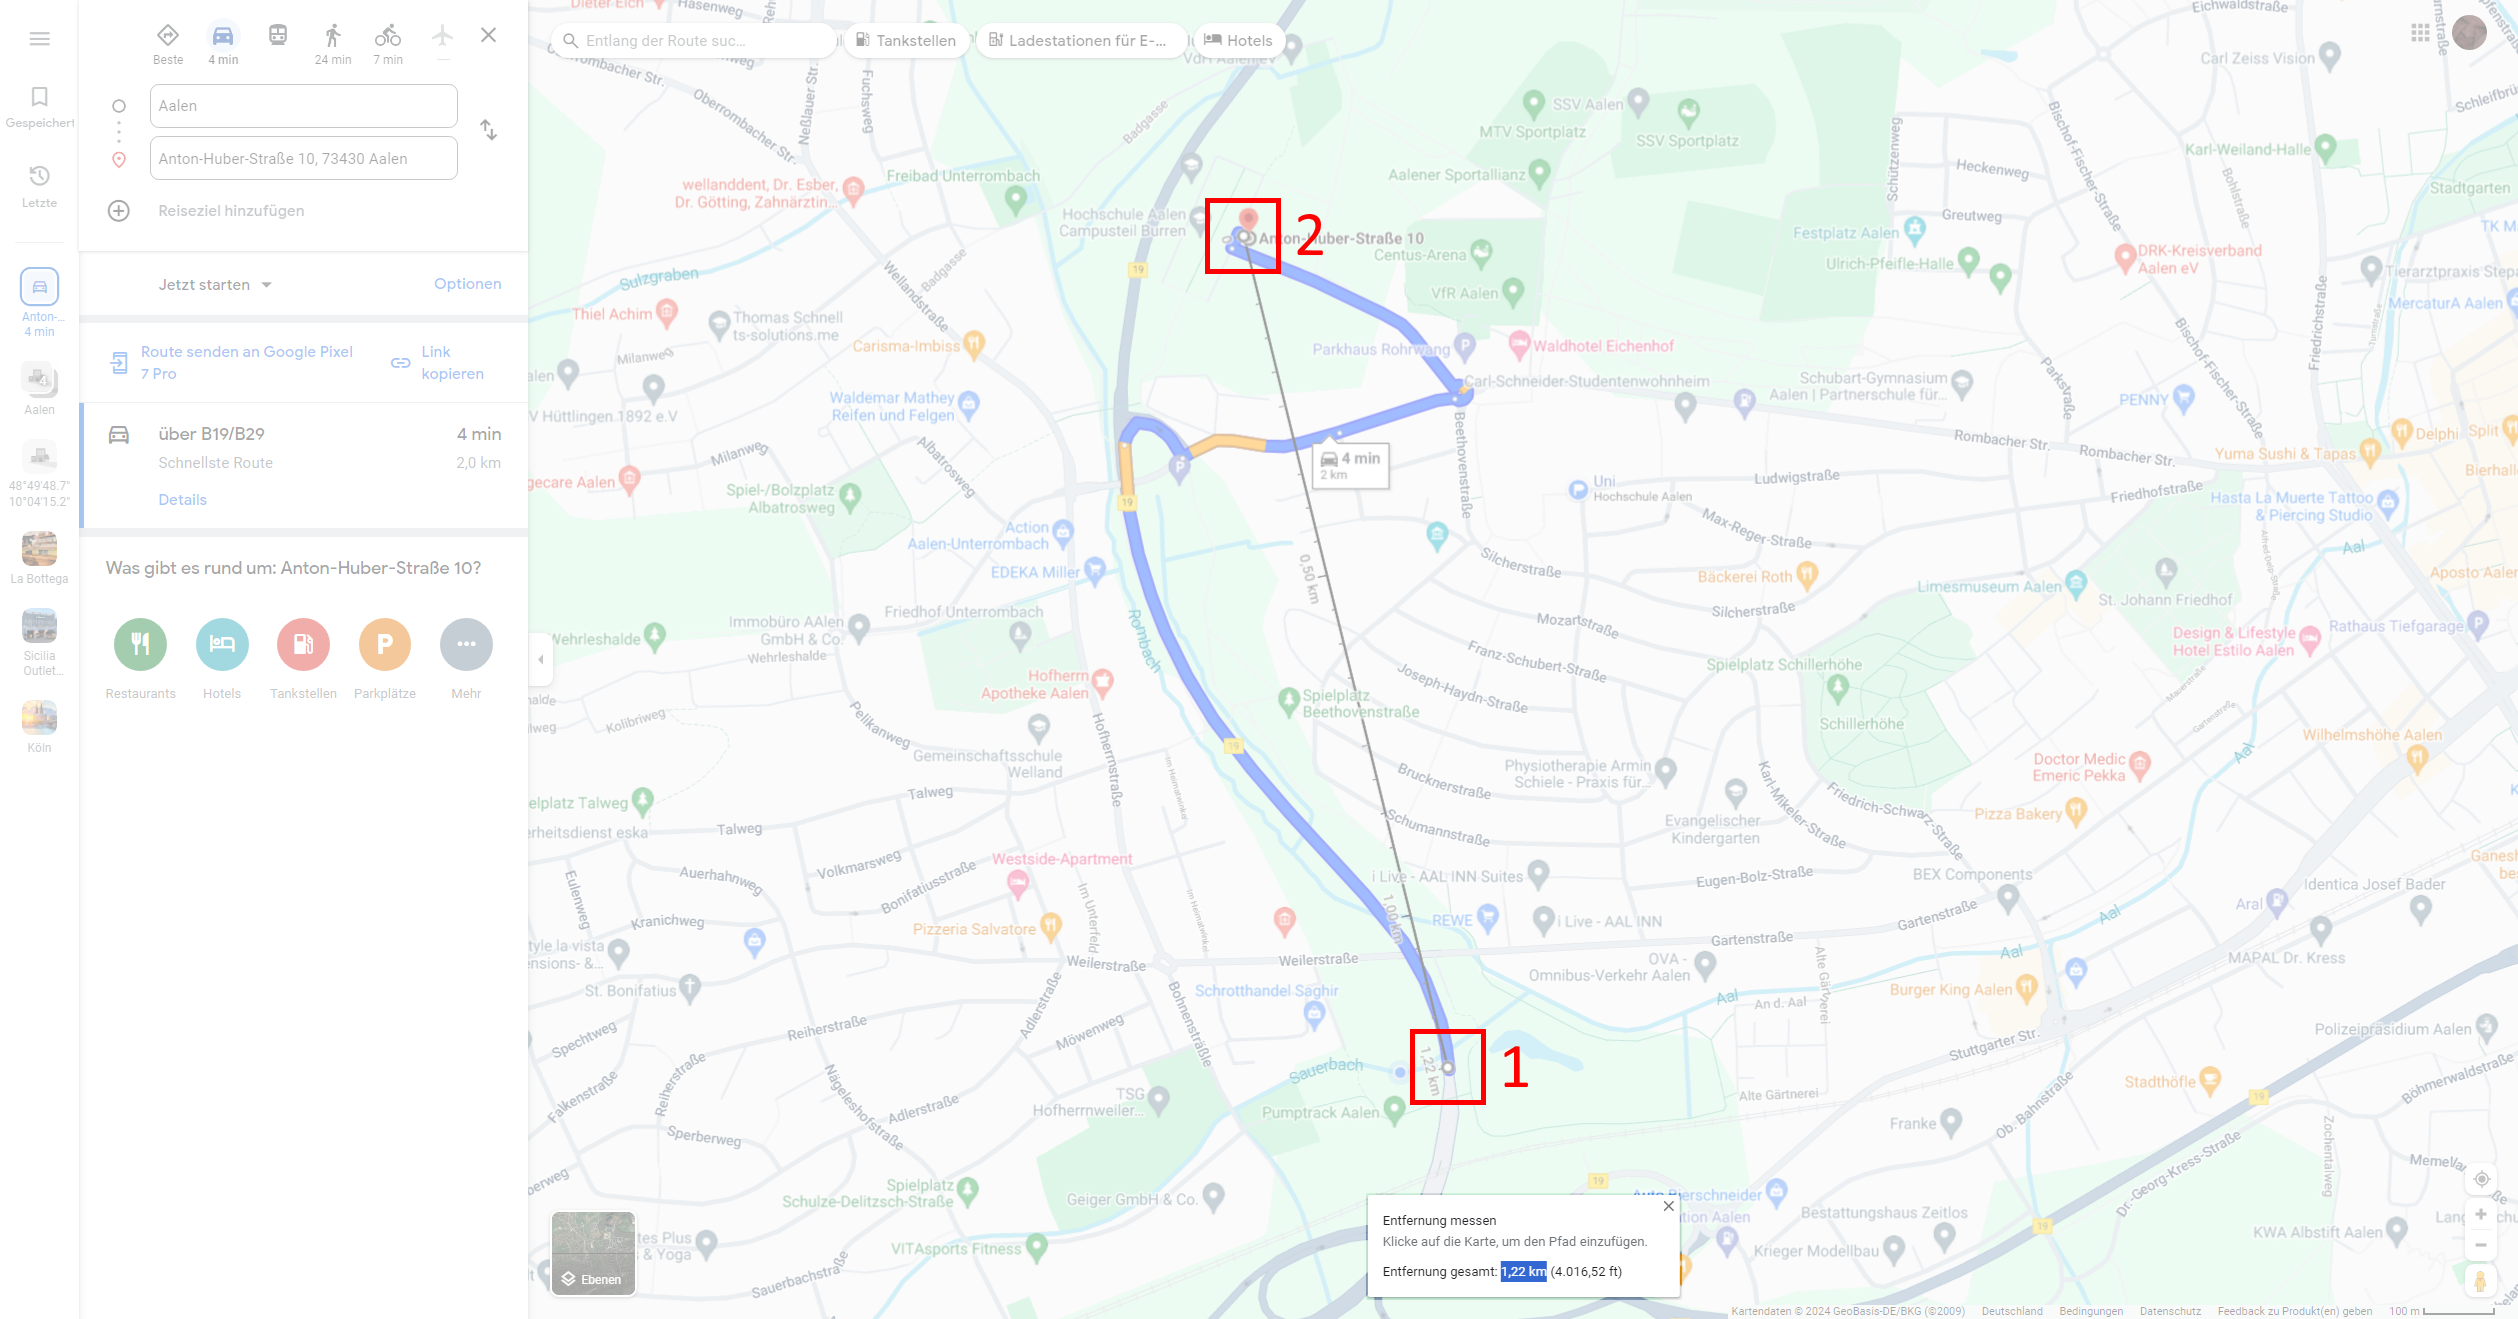
\includegraphics[width=\textwidth]{images/PrAr_Impl_Geolocation-Map.png}
    \caption{Bildschirmabschnitt Abstand Teilnehmer und Lösung}
    \label{fig:implementierung:geolocation_map}
\end{figure}

Abbildung \ref{fig:implementierung:geolocation_map} stellt den Standort des Teilnehmers (Abbildung \ref{fig:implementierung:geolocation_map} - 1) zu einem gesuchten Standort (Abbildung \ref{fig:implementierung:geolocation_map} - 2) dar. Die tatsächliche Distanz entspricht in diesem Beispiel \textit{1213.14} Meter.

\begin{figure}[H]
    \centering
    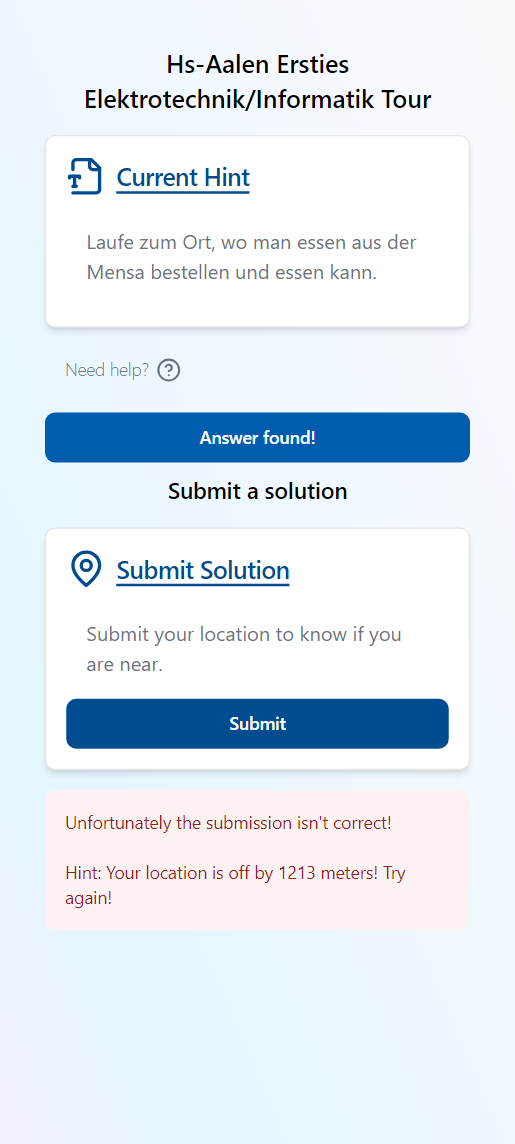
\includegraphics[width=0.5\textwidth]{images/PrAr_Impl_Geolocation-UI.png}
    \caption{Bildschirmabschnitt Abstands-Hinweis an Teilnehmer}
    \label{fig:implementierung:geolocation_ui}
\end{figure}

Abbildung \ref{fig:implementierung:geolocation_ui} zeigt den Zustand der Benutzeroberfläche an, nachdem ein Teilnehmer seine Position als Lösung an das System schickt. Es wurde korrekterweise erkannt, dass der Teilnehmer \textit{1213.14} Meter von der gewollten Lösung entfernt ist.

\subsection{Levenshtein-Algorithmus zur Bestimmung textueller Unterschiede}
Um den Nutzern Feedback darüber zu geben, wie nah ihre eingesandte Antwort an der korrekten Lösung liegt, wird neben der Haversine-Formel auch ein Algorithmus zur Berechnung der Levenshtein-Distanz eingesetzt. Diese Methode wird verwendet, wenn die Lösung aus Textdaten besteht, wie etwa bei der Eingabe von Textantworten auf Rätsel oder Aufgabenstellungen.

Die Levenshtein-Distanz misst den Unterschied zwischen zwei Zeichenketten in Bezug auf die minimale Anzahl von Einfüge-, Lösch- und Ersetzungsoperationen, die erforderlich sind, um die eine Zeichenkette in die andere zu transformieren. Dies ist besonders nützlich, um Tippfehler oder leichte Abweichungen in den Antworten der Nutzer zu identifizieren und entsprechende Rückmeldungen zu geben, die darauf hinweisen, dass die Antwort fast richtig ist, wenn nur geringe Abweichungen vorliegen.

Der folgende C\#-Code zeigt die Implementierung der Levenshtein-Distanz:
\newpage
\begin{lstlisting}[language=c,caption={Code Ausschnitt zum Levenshtein Distanz Algorithmus in C\#}]
public static int LevenshteinDistance(string givenText, string expectedText)
    {
        int n = givenText.Length;
        int m = expectedText.Length;
        int[,] d = new int[n + 1, m + 1];

        // Initialize the distance matrix
        for (int i = 0; i <= n; i++)
        {
            d[i, 0] = i;
        }
        for (int j = 0; j <= m; j++)
        {
            d[0, j] = j;
        }

        // Compute the distances
        for (int i = 1; i <= n; i++)
        {
            for (int j = 1; j <= m; j++)
            {
                int cost = (givenText[i - 1] == expectedText[j - 1]) ? 0 : 1;

                d[i, j] = Math.Min(
                    Math.Min(d[i - 1, j] + 1, d[i, j - 1] + 1),
                    d[i - 1, j - 1] + cost);
            }
        }

        return d[n, m];
    }
\end{lstlisting}
Die Matrix \lstinline{d} wird so initialisiert, dass die ersten Zeilen und Spalten mit aufsteigenden Werten gefüllt sind. Diese Werte entsprechen den Kosten für das Einfügen oder Löschen von Zeichen, um die Länge der anderen Zeichenkette zu erreichen. Die Hauptlogik des Algorithmus durchläuft die Matrix und berechnet die minimalen Kosten für die Transformation von Substrings. Dies geschieht durch den Vergleich der aktuellen Zeichen der beiden Zeichenketten und der Anwendung der entsprechenden Operationen (Einfügen, Löschen, Ersetzen). Der letzte Wert in der Matrix \lstinline{d[n, m]} gibt die minimale Anzahl der Transformationen an, die erforderlich sind, um die beiden Zeichenketten anzugleichen.

Die Levenshtein-Distanz ermöglicht es dem System, präzise Rückmeldungen zu geben, wie nahe der Nutzer an der richtigen Antwort ist, und unterstützt so ein positives Benutzererlebnis durch konstruktives Feedback.

\subsubsection{Anwendungsbeispiel des Levenshtein-Algorithmus}

Im Folgenden wird der Levenshtein-Algorithmus zum Bestimmen der Anzahl an abweichenden Ziffern zu einem gesuchten Lösungstext verwendet.

\begin{figure}[H]
    \centering
    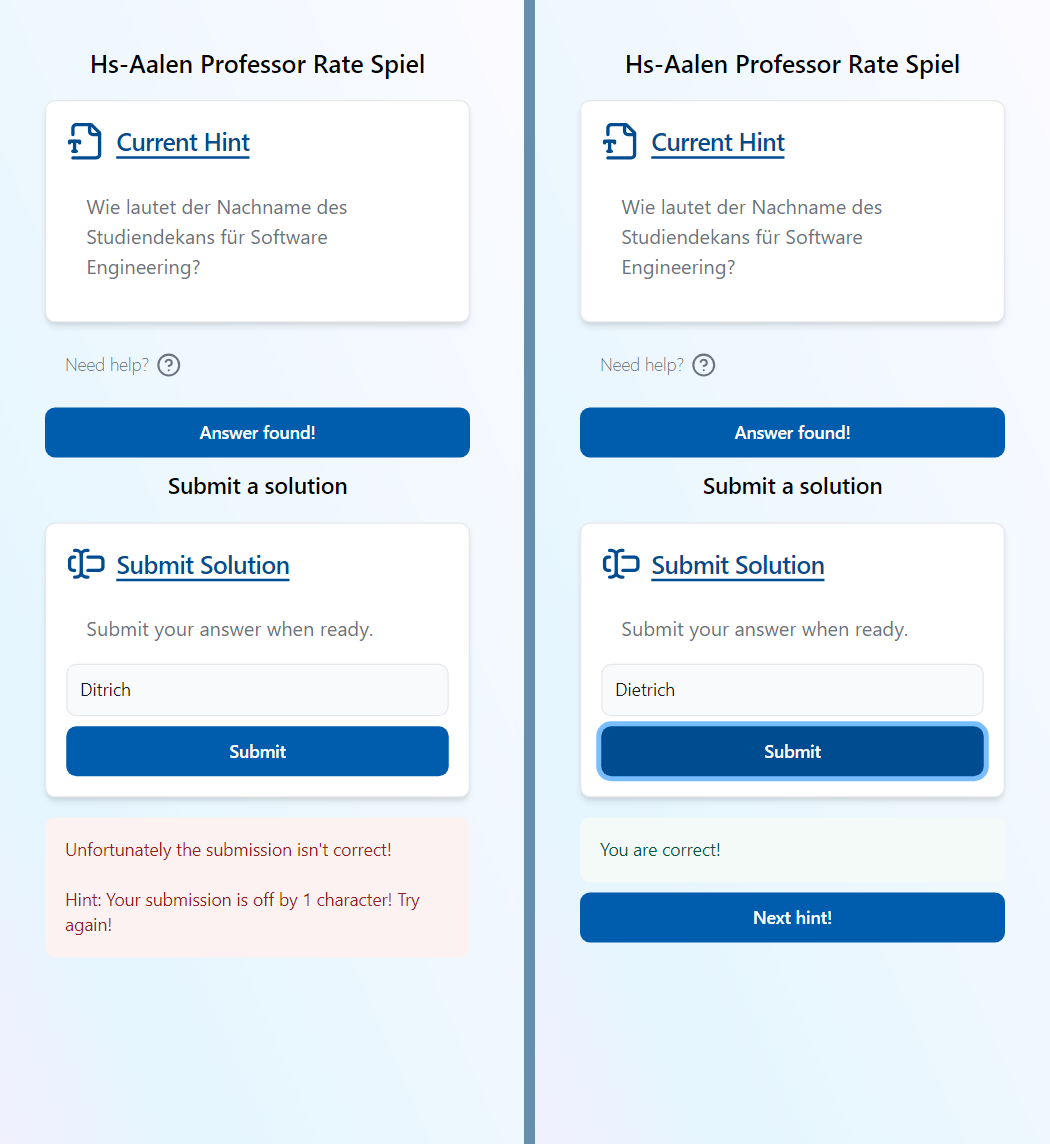
\includegraphics[width=0.75\textwidth]{images/PrAr_Impl_CharacterDiff-UI.png}
    \caption{Bildschirmabschnitte Text Unterschied an Teilnehmer}
    \label{fig:implementierung:characterdiff_ui}
\end{figure}

Der linke Bildschirmabschnitt in Abbildung \ref{fig:implementierung:characterdiff_ui} zeigt den Hinweis, wenn ein Teilnehmer sich bei seiner Lösung um eine Ziffer vertan hat. Der rechte Bildschirmabschnitt in Abbildung \ref{fig:implementierung:characterdiff_ui} wird angezeigt, wenn der Benutzer eine korrekte (Text-)Lösung eingegeben hat.

